\documentclass[a4paper,11pt]{article}
\usepackage{polski}
\usepackage[utf8]{inputenc}
\usepackage{latexsym}
\usepackage{graphicx} 
\usepackage{float}
\usepackage[margin=2cm]{geometry}
\usepackage{lscape}
\usepackage{listings}
\usepackage{color}
\usepackage{underscore}

\definecolor{mygreen}{rgb}{0,0.6,0}
\definecolor{mygray}{rgb}{0.5,0.5,0.5}
\definecolor{mymauve}{rgb}{0.58,0,0.82}

\lstset{ %
  backgroundcolor=\color{white},   % choose the background color; you must add \usepackage{color} or \usepackage{xcolor}; should come as last argument
  basicstyle=\footnotesize,        % the size of the fonts that are used for the code
  breakatwhitespace=false,         % sets if automatic breaks should only happen at whitespace
  breaklines=true,                 % sets automatic line breaking
  captionpos=b,                    % sets the caption-position to bottom
  commentstyle=\color{mygreen},    % comment style
  deletekeywords={...},            % if you want to delete keywords from the given language
  escapeinside={\%*}{*)},          % if you want to add LaTeX within your code
  extendedchars=true,              % lets you use non-ASCII characters; for 8-bits encodings only, does not work with UTF-8
  frame=single,	                   % adds a frame around the code
  keepspaces=true,                 % keeps spaces in text, useful for keeping indentation of code (possibly needs columns=flexible)
  keywordstyle=\color{blue},       % keyword style
  language=VHDL,                 % the language of the code
  morekeywords={*,...},            % if you want to add more keywords to the set
  numbers=left,                    % where to put the line-numbers; possible values are (none, left, right)
  numbersep=5pt,                   % how far the line-numbers are from the code
  numberstyle=\tiny\color{mygray}, % the style that is used for the line-numbers
  rulecolor=\color{black},         % if not set, the frame-color may be changed on line-breaks within not-black text (e.g. comments (green here))
  showspaces=false,                % show spaces everywhere adding particular underscores; it overrides 'showstringspaces'
  showstringspaces=false,          % underline spaces within strings only
  showtabs=false,                  % show tabs within strings adding particular underscores
  stepnumber=2,                    % the step between two line-numbers. If it's 1, each line will be numbered
  stringstyle=\color{mymauve},     % string literal style
  tabsize=2,	                   % sets default tabsize to 2 spaces
  title=\lstname,                  % show the filename of files included with \lstinputlisting; also try caption instead of title
  language=C++,
  literate={ą}{{\k{a}}}1
             {Ą}{{\k{A}}}1
             {ę}{{\k{e}}}1
             {Ę}{{\k{E}}}1
             {ó}{{\'o}}1
             {Ó}{{\'O}}1
             {ś}{{\'s}}1
             {Ś}{{\'S}}1
             {ł}{{\l{}}}1
             {Ł}{{\L{}}}1
             {ż}{{\.z}}1
             {Ż}{{\.Z}}1
             {ź}{{\'z}}1
             {Ź}{{\'Z}}1
             {ć}{{\'c}}1
             {Ć}{{\'C}}1
             {ń}{{\'n}}1
             {Ń}{{\'N}}1
}


\begin{document}

\begin{titlepage}

\newcommand{\HRule}{\rule{\linewidth}{0.5mm}}
\center
 
\textsc{\LARGE Politechnika Wrocławska}\\[1.5cm] 
\textsc{\Large Układy cyfrowe i systemy wbudowane}\\[0.5cm] %TU

\HRule \\[0.5cm]
{ \huge \bfseries Dokumentacja projektu \\ Organy z możliwością zapisywania i odtarzania melodii.}\\[0.5cm] %TU
\HRule \\[1.6cm]
 
%\begin{minipage}{0.4\textwidth}
\begin{flushleft} \large

\emph{Autorzy:}\\
Łukasz  \textsc{Bieszczad}\\ %TU
Krzysztof  \textsc{Buczak}\\ %TU

\end{flushleft}
%\end{minipage}

%\begin{minipage}{0.4\textwidth}
\begin{flushright} \large

\emph{Prowadzący:} \\
dr inż. Jarosław \textsc{Sugier} %TU

\end{flushright}
%\end{minipage}\\[4cm]

\vfill
{\large 18 maja 2018}\\[3cm] %TU %TU


\end{titlepage}

\tableofcontents
\newpage

\section{Wprowadzenie}
\subsection{Cel i zakres}
Celem projektu było stworzenie jednooktawowego "instrumentu" klawiszowego, obsługiwanego za pomocą klawiatury PS/2. Wciskanie poszczególnych klawiszy miało powodować odtwarzanie dźwięków przez podpięty do pinów głośniczek. Dodatkowo częścią zadania było także zaimplementowanie funkcjonalności nagrywania melodii (zapis do pamięci ROM) i odtwarzania nagranego materiału, a także wykorzystanie wyświetlacza LCD do pokazania stanu nagrywania i diody LED do przekazania informacji o trwającym właśnie nagrywaniu.

\subsection{Zagadnienia teoretyczne}

\subsection{Sprzęt}
Językiem projektu był język opisu sprzętu VHDL. Stanowisko laboratoryjne/projektowe zostało wyposażone w układ Spartan-3E oraz komputer z oprogramowaniem Xilinx ISE, pozwalającym kompilować kod VHDL pod dostarczony sprzęt, a także wykonywać symulacje testujące działanie systemu. Wykorzystaliśmy także port PS/2 (klawiatura symulująca keyboard), piny do podłączenia głośnika, ekran LCD wyświetlający stan nagrywania (pozostały czas) i układ pamięci ROM do przechowywania nagranych melodii.

\section{Projekt}
\subsection{Schemat i hierarchia projektu}
\begin{figure}[H]
\center
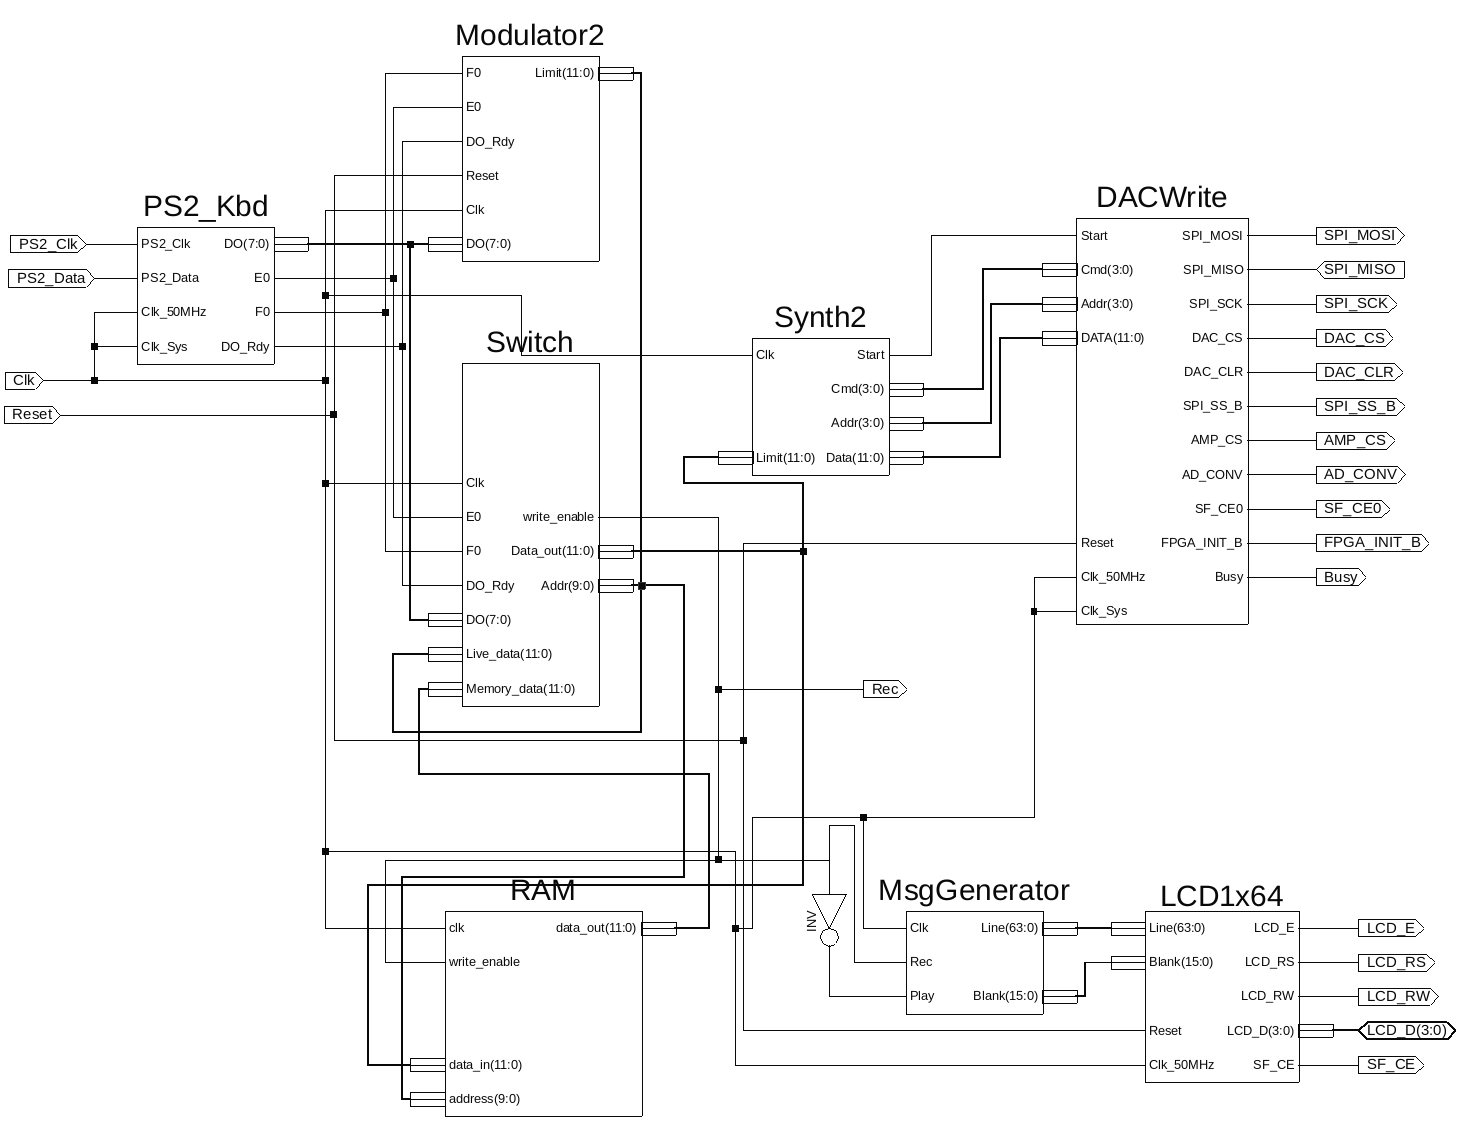
\includegraphics[scale=0.35]{schemat.png}
\caption{Schemat całego projektu.}
\end{figure}
\textbf{Hierarchia modułów:}
\begin{itemize}
\item schemat
\begin{itemize}
\item DACWrite
\item Modulator2
\item PS2_Kdb
\item Synth2
\item Switch
\item RAM
\item LCD1x64
\item MsgGenerator
\item ADC_DAC.ucf
\item GenIO.ucf
\item LCD.ucf
\end{itemize}
\end{itemize}

\subsection{Moduły}
W tym podrozdziale znajdują się opisy i symulacje modułów stworzonych na zajęciach w ramach projektu.

\subsubsection{Modulator2}
Ten moduł odpowiedzialny jest za wysyłanie wartości ograniczającej licznik w module Synth2 na podstawie sygnału pochodzącego z klawiatury. Jest oparty na maszynie stanów, która składa się 14 stanów odpowiadających różnym dźwiękom w oktawie lub ciszy. Wartości, które zwraca moduł na wyjściu zostały obliczone w taki sposób, aby przy częstotliwości 50 MHz licznik w następnym module generował falę piłokształtną o odpowiedniej dla danego dźwięku i stanu częstotliwości.

\begin{figure}[H]
\center
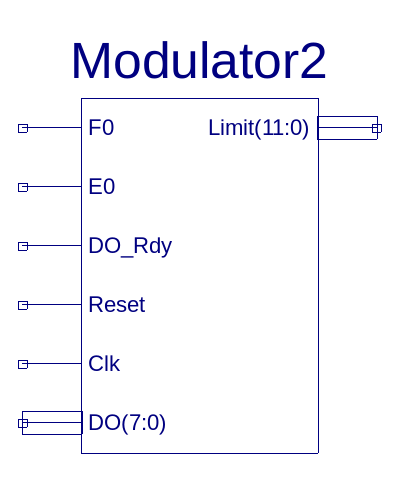
\includegraphics[scale=0.5]{modulatorSymb.png}
\caption{Symbol modułu Modulator2.}
\end{figure}

\subsubsection*{Wejścia modułu:}
\begin{itemize}
\item F0 - symbolizuje zwolnienie klawisza klawiatury
\item E0 - symbolizuje czy dane to tzw. kod rozszerzony
\item DO_Rdy - symbolizuje zakończenie odbierania kodu
\item Clk - symbolizuje zegar
\item DO[7:0] - symbolizuje otrzymane dane z klawiatury
\end{itemize}

\subsubsection*{Wyjścia modułu:}
\begin{itemize}
\item limit[11:0] - symbolizuje wartość graniczną dla licznika
\end{itemize}

\subsubsection*{Fragmenty kodu VHDL}
\begin{lstlisting}[caption=Procesy modułu Modulator2.]
architecture Behavioral of Modulator2 is
   type state_type is (Silence, C, Cis, D, Dis, E, F, Fis, G, Gis, A, Ais, H, C2);
   signal state, next_state: state_type;
begin

   process1 : process( Clk )
   begin
         if rising_edge( Clk ) then
            if Reset = '1' then
               state <= Silence;
            else
               state <= next_state;
            end if;
         end if;
   end process process1;
   
   process2: process (state, DO, F0, DO_Rdy)
   begin
      next_state <= state;
      
      if DO_Rdy = '1' and F0 = '0' then
      
         case state is
            when Silence =>
               if DO = X"1C" then
                  next_state <= C;
               elsif DO = X"1D" then
                  next_state <= Cis;
               elsif DO = X"1B" then
                  next_state <= D;
               elsif DO = X"24" then
                  next_state <= Dis;
               elsif DO = X"23" then
                  next_state <= E;
               elsif DO = X"2B" then
                  next_state <= F;
               elsif DO = X"2C" then
                  next_state <= Fis;
               elsif DO = X"34" then
                  next_state <= G;
               elsif DO = X"35" then
                  next_state <= Gis;
               elsif DO = X"33" then
                  next_state <= A;
               elsif DO = X"3C" then
                  next_state <= Ais;
              elsif DO = X"3B" then
                  next_state <= H;
              elsif DO = X"42" then
                  next_state <= C2;
              end if;
              
            when C =>
               next_state <= state;
               
            when Cis =>
               next_state <= state;
               
            when D =>
               next_state <= state;
               
            when Dis =>
               next_state <= state;
            
            when E =>
               next_state <= state;
               
            when F =>
               next_state <= state;
               
           when Fis =>
               next_state <= state;
               
           when G =>
               next_state <= state;
           
           when Gis =>
               next_state <= state;
               
            when A =>
               next_state <= state;
               
            when Ais =>
               next_state <= state;
               
            when H =>
               next_state <= state;
               
            when C2 =>
               next_state <= state;
         end case;
      elsif F0 = '1' then
         next_state <= Silence;
      end if;
   end process process2;
   
   with state select
      Limit <= X"5D4" when C,
               X"581" when Cis,
               X"532" when D,
               X"4E7" when Dis,
               X"4A1" when E,
               X"45E" when F,
               X"41F" when Fis,
               X"3E4" when G,
               X"3AC" when Gis,
               X"377" when A,
               X"345" when Ais,
               X"316" when H,
               X"2EA" when C2,
               X"000" when others;

end Behavioral;
\end{lstlisting}
Architektura jednostki na samym początku posiada deklarację wszystkich stanów, które odpowiadają dźwiękom w oktawie lub ciszy.
Pierwszy proces jest typowym przykładem procesu odpowiedzialnego za przełączanie stanu w maszynie stanów. Kolejny proces odpowiada za wybranie odpowiedniego stanu w zależności od wciśniętego klawisza. Ostatni element modułu to ustawianie odpowiedniego limitu w zależności od aktualnego stanu.

\subsubsection*{Graf maszyny stanu}
\begin{figure}[H]
\center
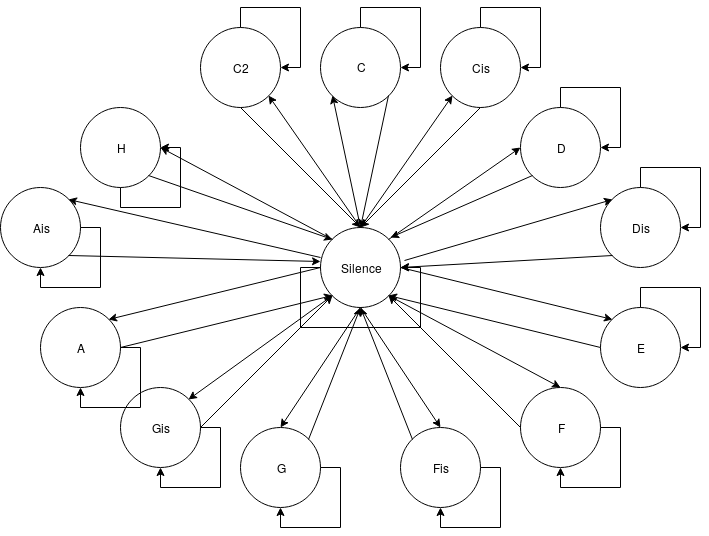
\includegraphics[scale=0.6]{modulatorMaszyna.png}
\caption{Graf maszyny stanów modułu Modulator2.}
\end{figure}

\subsubsection*{Symulacja}
\begin{figure}[H]
\center
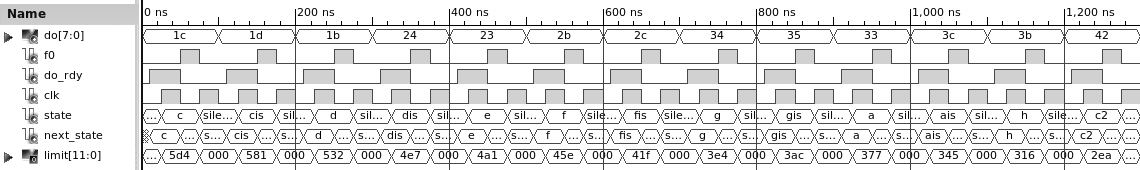
\includegraphics[scale=0.6]{modulatorsymbw.png}
\caption{Wyniki symulacji modułu Modulator2.}
\end{figure}
Na powyższej symulacji widać jak w momencie impulsu sygnału do_rdy z najbliższym taktem zegara zmieniany jest stan maszyny zgodnie z wciśniętym klawiszem oraz ustawiany jest odpowieni limit. W momencie impulsu f0 (puszczenie klawisza) stan przełączany jest na silence, a limit na wartość zerową.

\newpage
\subsubsection{Synth2}
Moduł ten odpowiada za generowanie fali piłokształtnej o odpowiedniej częstotliwości. Częstotliwość ta zależy od wartości limitu, którą moduł otrzymuje na wejściu.

\begin{figure}[H]
\center
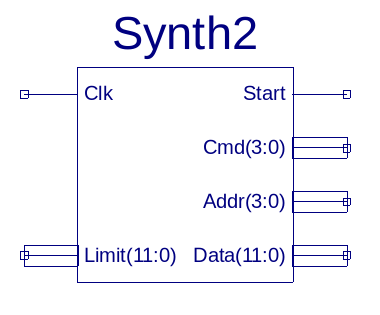
\includegraphics[scale=0.5]{synthsymb.png}
\caption{Symbol modułu Modulator2.}
\end{figure}

\subsubsection*{Wejścia modułu:}
\begin{itemize}
\item Clk - symbolizuje zegar
\item Limit[11:0] - symbolizuje limit dla wewnętrznego licznika
\end{itemize}

\subsubsection*{Wyjścia modułu:}
\begin{itemize}
\item Start - symbolizuje gotowość danych do przetworzenia przez DAC
\item Cmd - symbolizuje polecenie do wykonania
\item Addr - symbolizuje adres przetwornika DAC
\item Data[11:0] - symbolizuje dane do przetworzenia przez DAC
\end{itemize}

\subsubsection*{Fragmenty kodu VHDL}
\begin{lstlisting}[caption=Proces modułu Synth2.]
architecture Behavioral of Synth2 is
   signal count: UNSIGNED(11 downto 0) := X"000";
   signal waveCount: UNSIGNED(4 downto 0):= X"0"&'0';
   signal lmt: STD_LOGIC_VECTOR(11 downto 0) := X"000";
begin
   lmt <= Limit;
   process(Clk)
   begin
      if rising_edge(Clk) then
         count <= count + 1;
         start <= '0';
         if STD_LOGIC_VECTOR(count) = lmt then
            count <= X"000";
            waveCount <= waveCount + 1;
            start <= '1';
         end if;
      end if;
   end process;
   
   Data <= STD_LOGIC_VECTOR(waveCount)&"0000000";
   Cmd <= "0011";
   Addr <= "1111";
end Behavioral;

\end{lstlisting}
Moduł z każdym cyklem zegara zwiększa o jeden wartość wewnęrznego licznika, gdy licznik osiągnie limit zwiększany jest drugi licznik, który odpowiada generowanej fali. Wartość waveCount jest "doklejana" na początek wyjścia Data, aby osiągnąć większą amplitudę fali, czyli głośniejszy dźwięk. Komenda $Cmd <= "0011"$ oznacza natchmiastowe zaktualizowanie wartości na wybranym przetworniku o wskazaną wartość w $Data$. Natomiast adres $Addr <= "1111"$ oznacza wszystkie przetworniki na raz.

\subsubsection*{Symulacja}
\begin{figure}[H]
\center
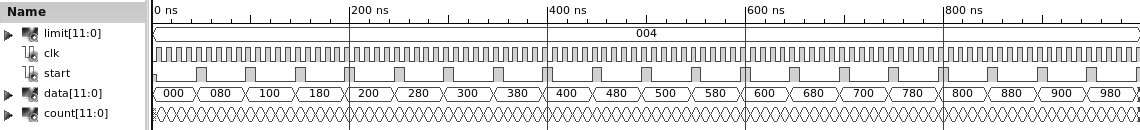
\includegraphics[scale=0.60]{synthsym1bw.png}
\caption{Wyniki symulacji modułu Synth2.}
\end{figure}
Symulacja została przeprowadzona dla $Limit <= X"004"$, co oznacza, że co 4 cykle zegara wartość $waveCount$ powinna się zwiększać, co za tym idzie wyjście $Data$ powinno również się zwiększać.

\begin{figure}[H]
\center
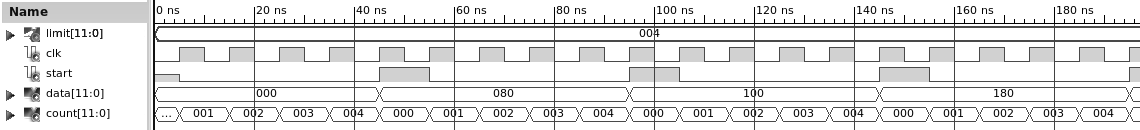
\includegraphics[scale=0.60]{synthsym2bw.png}
\caption{Wyniki symulacji modułu Synth2 w powiększeniu.}
\end{figure}

\subsubsection{Switch}
Moduł ten jest odpowiedzialny za zarządzanie trybem pracy urządzenia. Na podstawie danych otrzymywany z klawiatury decyduje, czy urządzenie powinno odtwarzać dźwięki według klawiszy zczytywanych z klawiatury, nagrywać dane do pamięci RAM, czy też odtwarzać melodię z pamięci. Jest oparty na prostej trójstanowej maszynie stanu: $None, Play, Rec$.

\begin{figure}[H]
\center
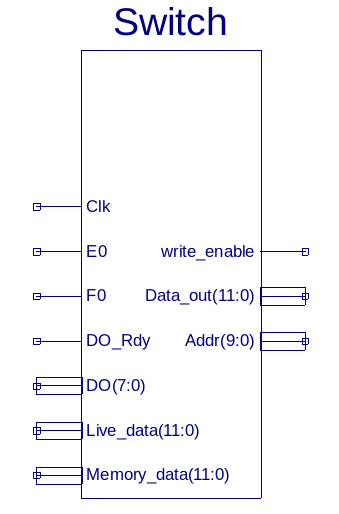
\includegraphics[scale=0.60]{switchsymb.png}
\caption{Symbol modułu Switch.}
\end{figure}

\subsubsection*{Wejścia modułu}
\begin{itemize}
\item Clk - symbolizuje zegar
\item F0 - symbolizuje zwolnienie klawisza klawiatury
\item E0 - symbolizuje czy dane to tzw. kod rozszerzony
\item DO_Rdy - symbolizuje zakończenie odbierania kodu
\item DO[7:0] - symbolizuje otrzymane dane z klawiatury
\item LiveData[11:0] - symbolizuje dane otrzymywane z modułu Synth2.
\item MemoryData[11:0] - symbolizuje dane otrzymywane z modułu RAM.
\end{itemize}

\subsubsection*{Wyjścia modułu}
\begin{itemize}
\item write_enable - symbolizuje pozowlenie na zapisywanie do pamięci RAM
\item Data_out[11:0] - symbolizuje wychodzące dane wybrane spośród LiveData lub MemoryData
\item Addr[11:0] - symbolizuje miejsce w pamięci RAM, z którego dane mają być wczytane lub do którego mają być zapisane.
\end{itemize}

\subsubsection*{Graf maszyny stanów}
\begin{figure}[H]
\center
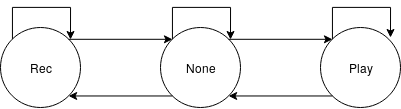
\includegraphics[scale=1]{switchmaszyna.png}
\caption{Graf maszyny stanów modułu Switch.}
\end{figure}
$Rec$ oznacza nagrywanie, $Play$ oznacza odtwarzania nagrania, a $None$ oznacza odtwarzanie tylko dźwięków odczytanych z klawiatury.

\subsubsection*{Fragmenty kodu VHDL}
\begin{lstlisting}
architecture Behavioral of Switch is
   type state_type is (None, Rec, Play);
   signal state, next_state: state_type;
   signal TmpAddr: UNSIGNED(9 downto 0) := X"00"&"00";
   signal count: UNSIGNED(19 downto 0) := X"00000";
  
begin
   process1 : process( Clk )
      begin
         if rising_edge( Clk ) then
            state <= next_state;
         end if;
   end process process1;
   
   process2: process (state, DO, F0, DO_Rdy)
   begin
      next_state <= state;
      
      if DO_Rdy = '1' and F0 = '0' then
         case state is
               when None =>
                  if DO = X"5A" then
                     next_state <= Play;
                  elsif DO = X"29" then
                     next_state <= Rec;
                  end if;
                  
               when Play =>
                  if DO = X"5A" then
                     next_state <= None;
                  end if;
                  
               when Rec =>
                  if DO = X"29" then
                     next_state <= None;
                  end if;
         end case;
      end if;
   end process;
               
   with state select
      write_enable <= '1' when Rec,
                      '0' when others;
                      
   with state select
      Data_out <= Live_data when Rec,
                  Memory_data when Play,
                  Live_data when None;
                      
   Addr <= STD_LOGIC_VECTOR(TmpAddr);
                      
   process3: process (state, clk)
   begin
      if rising_edge(clk) then
         if state = rec or state = play then
            count <= count + 1;
            if count = x"F4240" then
               TmpAddr <= TmpAddr + 1;
               count <=  X"00000";
            end if;
         else
            count <= X"00000";
            TmpAddr <= X"00"&"00";
         end if;
      end if;
   end process;
end Behavioral;
\end{lstlisting}
Pierwszy proces odpowiada za przechodzenie do następnego stanu. Drugi proces wybiera następny stan na podstawie wciśniętego klawisza. Moduł wybiera, który z $Live_data$ lub $Memory_data$ wysłać na wyjście w zależności od tego w jakim stanie się znajduje maszyna. Ostatni proces jest odpowiedzialny za przełączanie adresu co 0,02 sekundy w trakcie nagrywania lub odtwarzania nagrania oraz za zerowanie adresu w trybie $None$.

\subsubsection*{Symulacja}
\begin{figure}[H]
\center
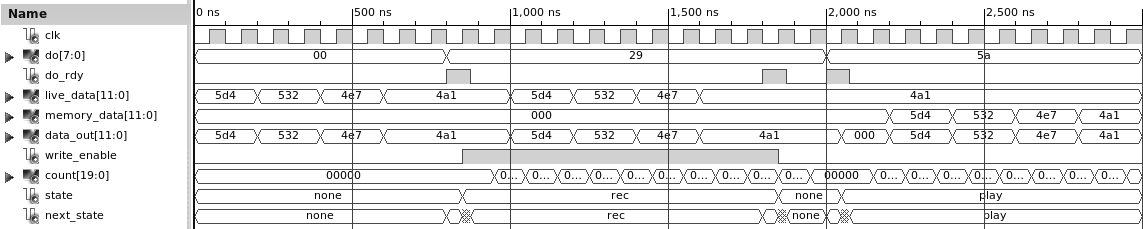
\includegraphics[scale=0.6]{switchsym1bw.png}
\caption{Symulacja modułu Switch cz.1.}
\end{figure}

\begin{figure}[H]
\center
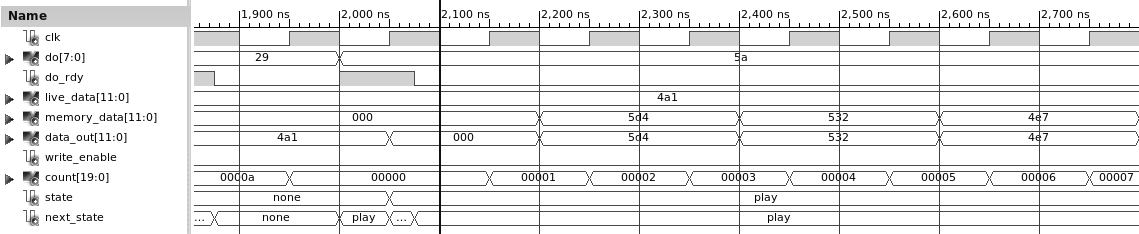
\includegraphics[scale=0.6]{switchsym2bw.png}
\caption{Symulacja modułu Switch cz.2.}
\end{figure}

Gdy stan maszyny jest w trybie $None$ na wyjście są wysyłane dane z $LiveData$ podobnie, w trybie $Rec$ z tą różnicą, że w trybie nagrywania dodatkowo aktywny jest sygnał $write_enable$, który pozwala na zapisywanie danych do pamięci RAM. W stanie $Play$ na wyjście modułu wysyłane są dane z wejscia $memory_data$, a $live_data$ jest ignorowane. Dodatkowo w trakcie nagrywania i odtwarzania zwiększa się licznik. Gdy osiągnie on wartość $X"F4240"$ czyli 1000000, zmienia się adres zapisu lub odczytu z modułu RAM. Dzięki temu, przy częstotliwości 50 MHz, sygnał jest próbkowany 50 razy w ciągu sekundy, czyli co 0,02s.

\subsubsection{RAM}
Jest to pamięć, która pozwala na zapisywanie i czytywanie danych.

\begin{figure}[H]
\center
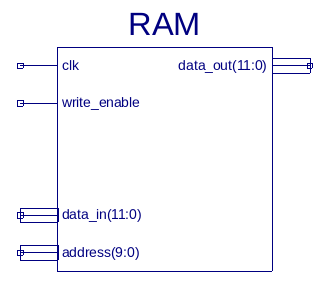
\includegraphics[scale=0.8]{ramsymb.png}
\caption{Symbol modułu RAM.}
\end{figure}

\subsubsection*{Wejścia modułu}
\begin{itemize}
\item clk - symbolizuje zegar
\item write_enable - symbolizuje pozwolenie na zapisywanie do pamięci
\item data_in[11:0] - symbolizuje dane do zapisania
\item address[9:0] - symbolizuje addres z którego należy czytać, lub do którego należy zapisywać dane
\end{itemize}

\subsubsection*{Wyjścia modułu}
\begin{itemize}
\item data_out[11:0] - symbolizuje dane wczytywane z pamięci.
\end{itemize}

\subsubsection*{Fragmenty kodu VHDL}
\begin{lstlisting}
architecture Behavioral of RAM is
   type ram_type is array (0 to 1023) of std_logic_vector (11 downto 0);                 
   signal memory : ram_type := (others => X"000");
begin
   process (clk)
   begin
      if (clk'event and clk = '1') then
         if (write_enable = '1') then
            memory(conv_integer(address)) <= data_in;
         end if;
         data_out <= memory(conv_integer(address));
      end if;
   end process;
end Behavioral;
\end{lstlisting}
Moduł w zależności od wartości $write_enable$ pozwala na zapisywanie lub wczytywanie z podanego na wejściu adresu.

\subsubsection{MsgGenerator}
Moduł ten odpowiada za wyświetlanie na ekranie wizualnej reprezentacji ile czasu pozostało do końca czasu nagrywania.

\begin{figure}[H]
\center
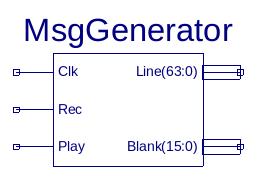
\includegraphics[scale=0.8]{msggen.png}
\caption{Symbol modułu MsgGenerator.}
\end{figure}

\subsubsection*{Wejścia modułu}
\begin{itemize}
\item Clk - symbolizuje zegar
\item Rec - symbolizuje tryb nagrywania
\item Play - symbolizuje tryb odtwarzania
\end{itemize}

\subsubsection*{Wyjścia modułu}
\begin{itemize}
\item Line[63:0] - symbolizuje dane wyjściowe na wyświetlaczu LCD
\item Blank[15:0] - symbolizuje które znaki mają być wyświetlane
\end{itemize}

\subsubsection*{Fragmenty kodu VHDL}
\begin{lstlisting}[caption=Procesy modułu MsgGenerator.]
architecture Behavioral of MsgGenerator is
   signal counter: UNSIGNED(27 downto 0) := X"0000000";
   signal show: UNSIGNED(3 downto 0) := X"0";
begin
   Line <= x"0000000000000000";
   process (Clk)
   begin
      if rising_edge(Clk) then
         if Rec = '1' then
            counter <= counter + 1;
            if counter = x"3d09000" then
                show <= show +1;
                counter <= X"0000000";
            end if;
         else
            counter <= X"0000000";
            show <= X"0";
         end if;
      end if;
   end process;
   
   with show select
       Blank <= X"0001" when X"0",
                X"0003" when X"1",
                X"0007" when X"2",
                X"000F" when X"3",
                X"001F" when X"4",
                X"003F" when X"5",
                X"007F" when X"6",
                X"00FF" when X"7",
                X"01FF" when X"8",
                X"03FF" when X"9",
                X"07FF" when X"A",
                X"0FFF" when X"B",
                X"1FFF" when X"C",
                X"3FFF" when X"D",
                X"7FFF" when X"E",
                X"FFFF" when X"F",
                X"0000" when others;     
end Behavioral;
\end{lstlisting}

Moduł wyświetla tylko same zera, jednak z biegnącym czasem kolejne zera znikają, co symbolizuje kończący się czas nagrywania.

\section{Implementacja}
\subsection{Zasoby}
\subsection{"User manual" urządzenia}

\section{Podsumowanie}
Zadanie udało się zrealizować w całości. Instrument jest w pełni działający, a ze względu na jasny podział na moduły można bez trudu dopisywać do niego kolejne funkcjonalności. Także sama wartość "merytoryczna" keyboarda nie pozostawia wiele do życzenia, ponieważ faktycznie pokrywa on całą oktawę, a wysokości dźwięków różnią się od siebie dokładnie tak jak w prawdziwym instrumencie, dzięki czemu mając nuty do utworu muzycznego możemy go zagrać.

\section{Literatura}

\end{document}

